\section{Wie verändert man den Levelaufbau? - Metatilemanipulation}

\subsection{Ziel}

Unser Ziel ist es ein Leveleditor zu erstellen, bei dem wir jeden Raum des ersten Levels individuell verändern können.
Es soll möglich sein die Metatiles einzelnt verändern zu können und somit die Möglichkeit hat, ein komplett neues eigenes Level zu erstellen.

\subsection{Methodik}

Durch Durchsuchen des WRAM's fanden wir folgenden Bereich: 0xCA00 - 0xCC3F. Dort ist der aktuell geladene Raum gespeichert, welcher aus einem
9x10 Metatiles Feld besteht.
Es wird abwechselnd das Metatile von der Oberwelt und das Metatile von der Unterwelt gespeichert. 
Beim betreten eines Raumes wird die Funktion fcn.1ea2 aufgerufen, welche alle Werte im genannten Bereich auf die entsprechende Metatile-ID setzt.
Beim zurückverfolgen der Werte fanden wir heraus wo die Räume gespeichert sind. Die Metatile-ID's der Räume im ersten Level sind in 
der 29. Rombank gespeichert, im Bereich folgender virtuellen Adressen: 0x001c414d - 0x001c4c8c. Wenn man mithilfe von Radare2 den Hexdump richtig 
formatiert, entsteht folgende Ausgabe:

\begin{figure}[H]
    \centering
    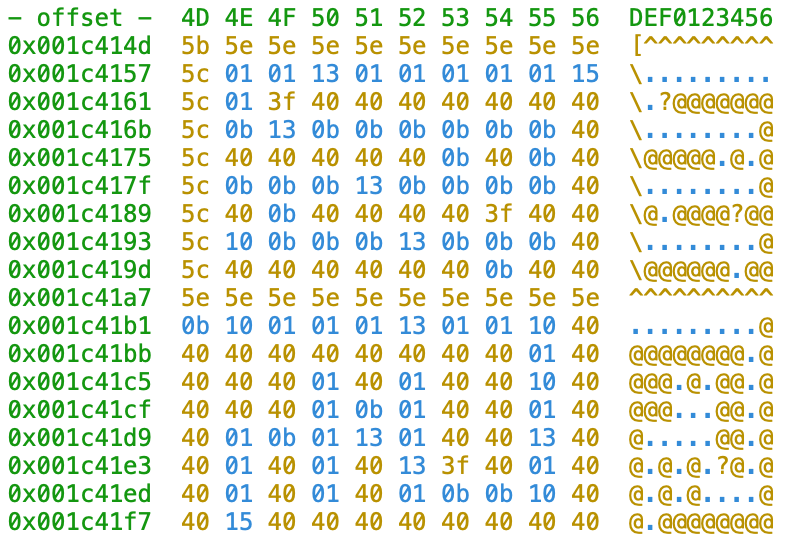
\includegraphics[width=0.8\linewidth]{Bilder/Metatileausgabe.png}
    \caption{2 Räume als hexdump}
    \label{fig:enter-label}
\end{figure}

Bei der Ausgabe kann man an der rechten Spalte, welche eine extended Ascii Interpretation ist, 
gut zwei Räume sehen.

\subsection{Ergebnis}
Wir erstellten einen Leveleditor, damit kann man jeden einzelnen Raum des ersten Levels individuell
verändern.
Er sieht folgendermaßen aus:

\begin{figure}[H]
    \centering
    % Erstes Bild
    \begin{minipage}{0.45\linewidth}
        \centering
        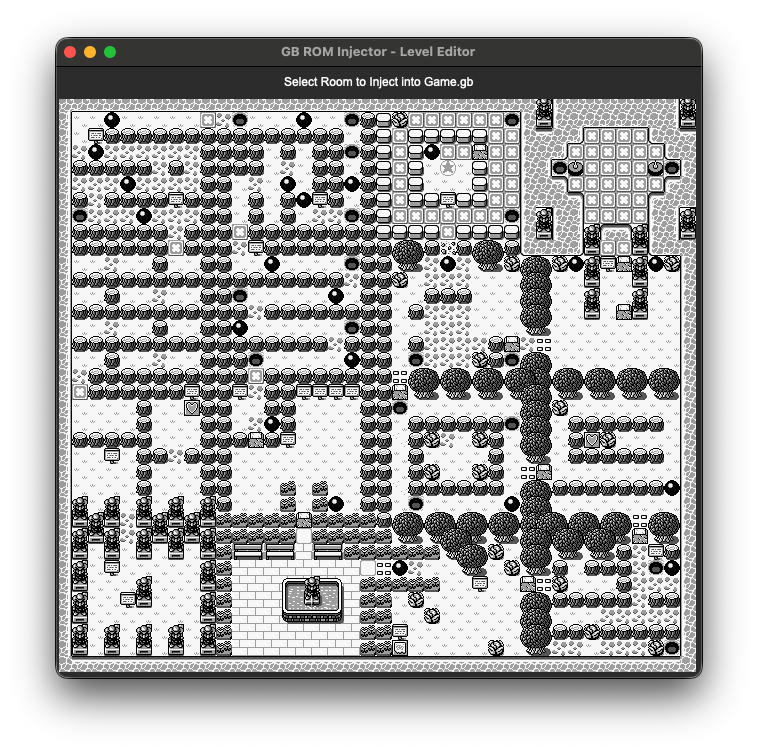
\includegraphics[width=\linewidth]{Bilder/Roomeditor1.png}
        \caption{erstes Fenster}
        \label{fig:enter-label}
    \end{minipage}
    \hfill
    % Zweites Bild
    \begin{minipage}{0.45\linewidth}
        \centering
        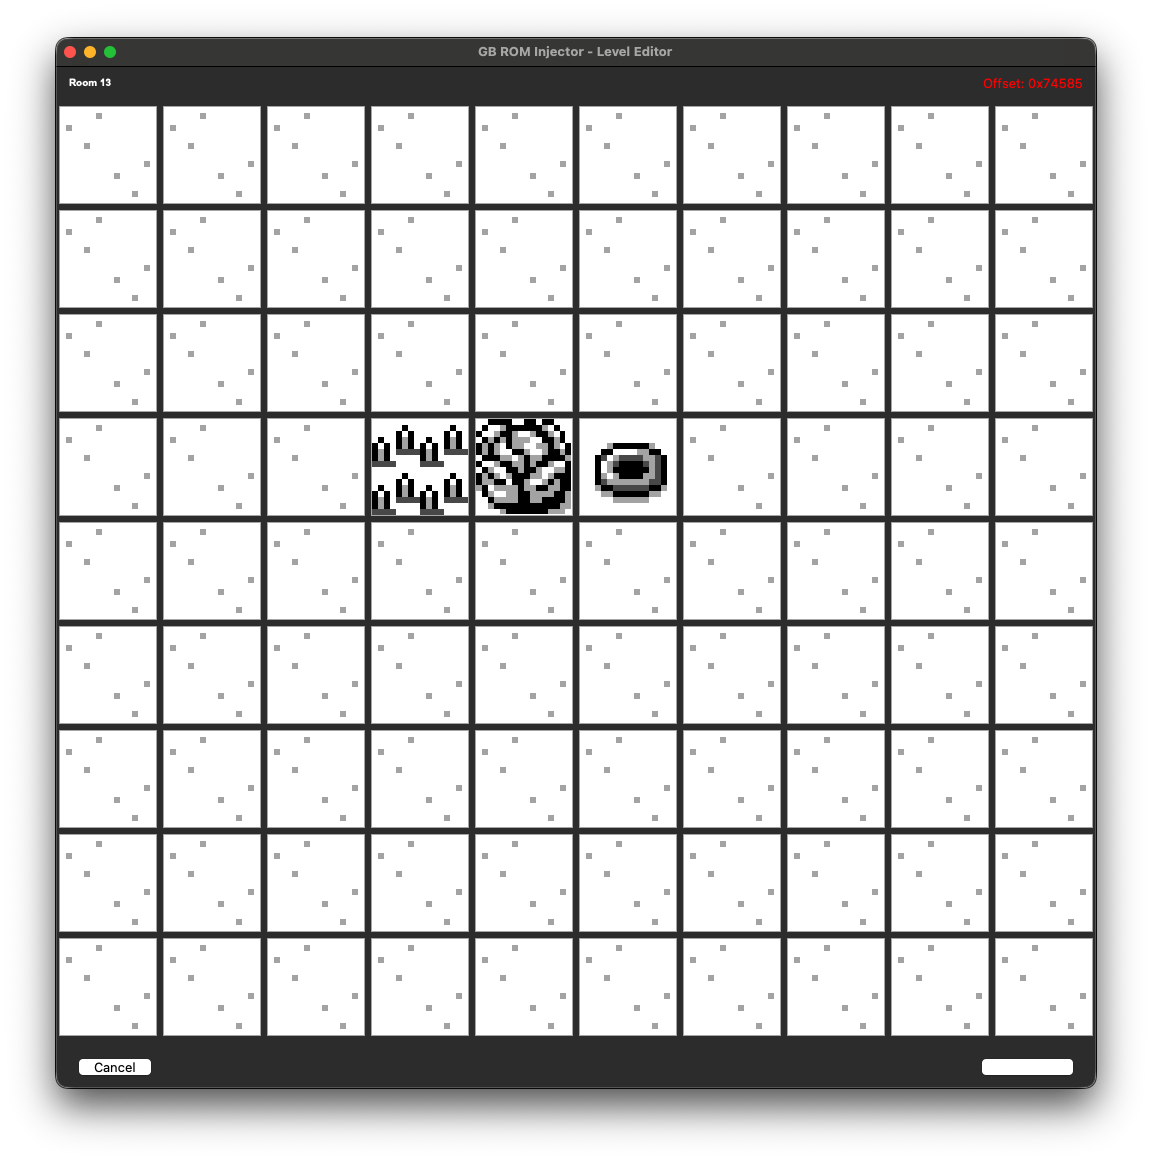
\includegraphics[width=\linewidth]{Bilder/Roomeditor2.png}
        \caption{zweites Fenster}
        \label{fig:enter-label}
    \end{minipage}
\end{figure}